% !TeX program = xelatex
\documentclass[a4paper,10pt]{article}

% ============================================================================
% សន្លឹកកិច្ចការសិស្ស ស-ខ្មៅ (Student Fill-In Worksheet — No-LCD Classroom)
% មេរៀនទី១៧ (១៧.៣)៖ ការគណនាមាឌនៃពីរ៉ាមីត (ត្រូវគ្នា ១០០% នឹង LS_Plan_PYR_VOL.tex)
% ============================================================================
\usepackage[a4paper, left=0.95cm, right=0.95cm, top=0.75cm, bottom=0.90cm, footskip=0.48cm]{geometry}
\usepackage{amsmath}
\usepackage{unicode-math}
\usepackage{fontspec}
\usepackage{array, colortbl}
\usepackage[table]{xcolor}
\usepackage{enumitem}
\usepackage{pifont}
\usepackage{fancyhdr}
\usepackage{lastpage}
\usepackage{tikz}
\usepackage[most]{tcolorbox}
\usetikzlibrary{calc, arrows.meta, angles, quotes, patterns, decorations.markings, babel}

\makeatletter
\let\@expl@@@mark@update@singlecol@structures@@\relax
\makeatother

\providecommand{\NGSFindFonts}{%
  \IfFileExists{C:/Windows/Fonts/cambria.ttc}{%
    \def\NGSSysPath{C:/Windows/Fonts/}%
    \def\NGSUserPath{C:/Users/KIT/AppData/Local/Microsoft/Windows/Fonts/}%
  }{%
    \IfFileExists{./fonts/KhmerOSsiemreap.ttf}{\def\NGSSysPath{./fonts/}\def\NGSUserPath{./fonts/}}{%
    \IfFileExists{../fonts/KhmerOSsiemreap.ttf}{\def\NGSSysPath{../fonts/}\def\NGSUserPath{../fonts/}}{%
    \IfFileExists{../../fonts/KhmerOSsiemreap.ttf}{\def\NGSSysPath{../../fonts/}\def\NGSUserPath{../../fonts/}}{%
    \IfFileExists{../../../fonts/KhmerOSsiemreap.ttf}{\def\NGSSysPath{../../../fonts/}\def\NGSUserPath{../../../fonts/}}{%
    \IfFileExists{../../../../fonts/KhmerOSsiemreap.ttf}{\def\NGSSysPath{../../../../fonts/}\def\NGSUserPath{../../../../fonts/}}{%
    \IfFileExists{../../../../../fonts/KhmerOSsiemreap.ttf}{\def\NGSSysPath{../../../../../fonts/}\def\NGSUserPath{../../../../../fonts/}}{%
    \IfFileExists{../../../../../../fonts/KhmerOSsiemreap.ttf}{\def\NGSSysPath{../../../../../../fonts/}\def\NGSUserPath{../../../../../../fonts/}}{%
      \def\NGSSysPath{../../../../../../../fonts/}\def\NGSUserPath{../../../../../../../fonts/}%
    }}}}}}}%
  }%
}
\NGSFindFonts

\setmathfont[Path={\NGSSysPath}, FontIndex=1, Scale=1.02]{cambria.ttc}
\defaultfontfeatures{Ligatures=TeX}

\setmainfont[
  Path={\NGSUserPath},
  Extension=.ttf,
  Script=Khmer,
  BoldFont={KhmerOSsiemreap},
  BoldFeatures={FakeBold=1.8},
  ItalicFont={KhmerOSsiemreap},
  ItalicFeatures={FakeSlant=0.25},
  BoldItalicFont={KhmerOSsiemreap},
  BoldItalicFeatures={FakeBold=1.8, FakeSlant=0.25}
]{KhmerOSsiemreap}

\newfontfamily\muol[Path={\NGSUserPath}, Extension=.ttf, Script=Khmer]{KhmerOSmuollight}
\newfontfamily\TimesEn[Path={\NGSSysPath}, Extension=.ttf, BoldFont={timesbd}, ItalicFont={timesi}, BoldItalicFont={timesbi}]{times}

\XeTeXlinebreaklocale "km"
\XeTeXlinebreakskip = 0pt plus 1pt minus 0.1pt

\definecolor{panelgray}{gray}{0.93}
\definecolor{headgray}{gray}{0.85}

\pagestyle{fancy}
\fancyhf{}
\renewcommand{\headrulewidth}{0pt}
\fancyfoot[L]{\fontsize{8pt}{10pt}\selectfont អនុវិទ្យាល័យព្រះក្រសាំង \en{---} គណិតវិទ្យា ថ្នាក់ទី៨ \en{|} មេរៀនទី១៧ (១៧.៣ ការគណនាមាឌនៃពីរ៉ាមីត)}
\fancyfoot[R]{\fontsize{8.2pt}{10pt}\selectfont ទំព័រ \en{\thepage\ / \pageref{LastPage}}}

\setlength{\parindent}{0pt}
\setlength{\parskip}{0pt}
\setlength{\tabcolsep}{4pt}

\newcommand{\en}[1]{{\TimesEn #1}}
\newcommand{\enbf}[1]{{\TimesEn\textbf{#1}}}
\newcommand{\unit}[1]{\,\text{\en{#1}}}
\newcommand{\cnum}[1]{\mbox{\fontsize{10pt}{12pt}\selectfont\ding{\numexpr181+#1\relax}}}
\newcommand{\chkbox}{\tikz[baseline=-0.15ex]\draw[black, line width=0.85pt] (0,0) rectangle (0.25cm,0.25cm);}
\newcommand{\blank}[1]{\makebox[#1]{\dotfill}}
\newcommand{\tri}[1]{\ensuremath{\triangle #1}}

\newcommand{\rightbox}[4][0.18]{%
  \draw[black, line width=0.8pt]
    ($(#3)!#1!(#2)$) -- ($($(#3)!#1!(#2)$)+($(#3)!#1!(#4)$)-(#3)$) -- ($(#3)!#1!(#4)$);
}

\newcommand{\secbar}[2]{%
  \vspace{3pt}%
  \begin{tcolorbox}[
    enhanced, sharp corners, colback=headgray, colframe=black,
    boxrule=0.9pt, boxsep=1pt, top=2.5pt, bottom=2.5pt, left=6pt, right=6pt,
    after skip=3pt
  ]
    {\muol\fontsize{9.2pt}{13.5pt}\selectfont #1}\hfill{\fontsize{8.3pt}{11.5pt}\selectfont\textbf{#2}}
  \end{tcolorbox}%
}

\newcolumntype{L}[1]{>{\raggedright\arraybackslash}p{#1}}
\newcolumntype{C}[1]{>{\centering\arraybackslash}p{#1}}

\begin{document}
\fontsize{9.4pt}{13.8pt}\selectfont

% ============================================================================
% ទំព័រទី ១៖ ក្បាលសន្លឹកកិច្ចការ + E1 (ប៉មទី១៧) + E2 (សមាមាត្រ 1/3 & គំរូទី 1, 2) + E3 (រូបមន្ត h vs d)
% ============================================================================
\begin{tcolorbox}[
  enhanced, sharp corners, colback=white, colframe=black,
  boxrule=1.1pt, boxsep=2.5pt, top=6pt, bottom=6pt, left=6pt, right=6pt, after skip=8pt
]
  \begin{center}
    {\muol\fontsize{10pt}{14.5pt}\selectfont សន្លឹកកិច្ចការសិស្ស \enbf{---} គណិតវិទ្យា ថ្នាក់ទី៨ \enbf{(}១៧\enbf{.}៣ ការគណនាមាឌនៃពីរ៉ាមីត\enbf{)}}\\[3.5pt]
    {\fontsize{8.8pt}{12pt}\selectfont
    ឈ្មោះសិស្ស / ដៃគូ៖ \blank{6.2cm} \hspace{0.2cm}
    ថ្នាក់៖ \blank{1.4cm} \hspace{0.2cm}
    ក្រុម៖ \blank{1.2cm} \hspace{0.2cm}
    កាលបរិច្ឆេទ៖ \blank{2.8cm}}
  \end{center}
\end{tcolorbox}

% --- E1 Engage: Architectural Tower Mystery (Ex #17 p. 229) ---
\begin{tcolorbox}[
  enhanced, sharp corners, colback=panelgray, colframe=black,
  boxrule=0.8pt, boxsep=2.5pt, top=6pt, bottom=6pt, left=6pt, right=6pt, after skip=8pt
]
  \textbf{បេសកកម្មទី១ (\en{E1 - Engage / POE})៖ ការប៉ាន់ស្មានមាឌដំបូលកំពូលប៉មរាងពីរ៉ាមីត (លំហាត់ទី១៧ ទំព័រ ២២៩)}\\[3pt]
  ប៉មមួយមានបាតជាការេជ្រុង $5\unit{m}$ ($B = 25\unit{m}^2$) ជញ្ជាំងឈររាងប្រអប់កែងកម្ពស់ $20\unit{m}$ និងដំបូលកំពូលរាងពីរ៉ាមីតដែលធ្វើឱ្យកម្ពស់សរុបស្មើ $24\unit{m}$ ($h_{\text{ដំបូល}} = 4\unit{m}$) ។ បើប្រអប់កែងដែលមានបាត $25\unit{m}^2$ និងកម្ពស់ $4\unit{m}$ មានមាឌ $100\unit{m}^3$ តើដំបូលពីរ៉ាមីតមានមាឌប៉ុន្មាន?\\[3pt]
  \ding{226}\ ទស្សន៍ទាយជាដៃគូមុនរៀន៖ \;\chkbox\ $100\unit{m}^3$ (ស្មើប្រអប់កែង) \hspace{0.4cm} \chkbox\ $50\unit{m}^3$ ($\frac{1}{2}$ នៃប្រអប់កែង) \hspace{0.4cm} \chkbox\ $\frac{100}{3}\unit{m}^3$ ($\frac{1}{3}$ នៃប្រអប់កែង)
\end{tcolorbox}

% --- E2 Explore Part A: 3-to-1 Sand Comparison & 6-Pyramid Cube Decomposition (p. 224) ---
\secbar{ផ្នែកទី១ \enbf{(}ក\enbf{)} ៖ សមាមាត្រ ៣\enbf{-}ទល់\enbf{-}១ រវាងព្រីសនិងពីរ៉ាមីត និងការបំបែកគូប \enbf{(E2 - Explore)}}{ការងារជាដៃគូ \en{5 min}}

\noindent
\begin{minipage}[c]{8.2cm}
  \centering
  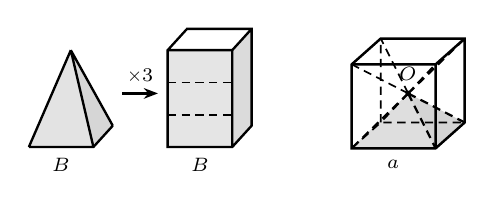
\begin{tikzpicture}[scale=0.82, every node/.style={font=\scriptsize, text=black}]
    % (1) ពីរ៉ាមីត x 3 = ព្រីស (ទំ.២២៤)
    \begin{scope}[shift={(-2.35,0)}]
      \coordinate (A) at (-1.35,-0.75);
      \coordinate (B) at (-0.35,-0.75);
      \coordinate (C) at (-0.05,-0.42);
      \coordinate (V) at (-0.70,0.75);
      \fill[gray!22] (A) -- (B) -- (V) -- cycle;
      \fill[gray!32] (B) -- (C) -- (V) -- cycle;
      \draw[black, line width=0.85pt] (A) -- (B) -- (C) (V) -- (A) (V) -- (B) (V) -- (C);
      \node[below=0.5pt] at (-0.85,-0.75) {$B$};
      \draw[-{Stealth[length=1.8mm]}, line width=0.85pt] (0.10,0.08) -- (0.65,0.08) node[midway, above=0.5pt] {$\times 3$};
      \coordinate (P) at (0.80,-0.75);
      \coordinate (Q) at (1.80,-0.75);
      \coordinate (R) at (2.10,-0.42);
      \coordinate (P1) at (0.80,0.75);
      \coordinate (Q1) at (1.80,0.75);
      \coordinate (R1) at (2.10,1.08);
      \coordinate (S1) at (1.10,1.08);
      \fill[gray!20] (P) -- (Q) -- (Q1) -- (P1) -- cycle;
      \fill[gray!28] (Q) -- (R) -- (R1) -- (Q1) -- cycle;
      \draw[black, line width=0.6pt, densely dashed] (0.80,-0.25) -- (1.80,-0.25) (0.80,0.25) -- (1.80,0.25);
      \draw[black, line width=0.85pt] (P) -- (Q) -- (R) -- (R1) -- (S1) -- (P1) -- cycle (P1) -- (Q1) -- (R1) (Q) -- (Q1);
      \node[below=0.5pt] at (1.30,-0.75) {$B$};
    \end{scope}

    % (2) គូបទ្រនុង a បំបែកជា 6 ពីរ៉ាមីតប៉ុនគ្នាត្រង់ផ្ចិត O
    \begin{scope}[shift={(2.15,-0.02)}]
      \coordinate (A) at (-0.85,-0.75);
      \coordinate (B) at (0.45,-0.75);
      \coordinate (C) at (0.90,-0.35);
      \coordinate (D) at (-0.40,-0.35);
      \coordinate (A1) at (-0.85,0.55);
      \coordinate (B1) at (0.45,0.55);
      \coordinate (C1) at (0.90,0.95);
      \coordinate (D1) at (-0.40,0.95);
      \coordinate (O) at (0.025,0.10);
      \fill[gray!26] (A) -- (B) -- (O) -- cycle;
      \fill[gray!34] (B) -- (C) -- (O) -- cycle;
      \draw[black, line width=0.6pt, densely dashed] (A) -- (D) -- (C) (D) -- (D1) (O) -- (D) (O) -- (A1) (O) -- (D1);
      \draw[black, line width=0.8pt, densely dashed] (O) -- (A) (O) -- (B) (O) -- (C) (O) -- (B1) (O) -- (C1);
      \draw[black, line width=0.9pt] (A) -- (B) -- (C) -- (C1) -- (D1) -- (A1) -- cycle (A1) -- (B1) -- (C1) (B) -- (B1);
      \fill (O) circle (1.2pt) node[above=1pt] {$O$};
      \node[below=0.5pt] at (-0.20,-0.75) {$a$};
    \end{scope}
  \end{tikzpicture}
\end{minipage}%
\hfill
\begin{minipage}[c]{10.4cm}\raggedright
  \textbf{ពិនិត្យដ្យាក្រាមពិសោធន៍ទំ.២២៤ និងការបំបែកគូបទ្រនុង $a$៖}\\[5.5pt]
  $1.$ ចាក់ខ្សាច់ពេញពីរ៉ាមីតចូលក្នុងព្រីស (បាត $B$ និងកម្ពស់ $h$ ស្មើគ្នា) ត្រូវចាក់ \blank{0.9cm} ដង\\
  \hspace*{0.3cm}ទើបពេញព្រីស $\Rightarrow 3 \cdot V_{\text{ពីរ៉ាមីត}} = B \cdot h \Rightarrow V_{\text{ពីរ៉ាមីត}} = \blank{1.8cm}$ ។\\[5pt]
  $2.$ \textbf{ផ្ទៀងផ្ទាត់តាមគូបទ្រនុង $a$ (មាឌ $a^3$)៖} ផ្ចិត $O$ បំបែកគូបជាពីរ៉ាមីតប៉ុនគ្នាចំនួន $6$\\
  \hspace*{0.3cm}ដែលមួយៗមានផ្ទៃបាត $B = a^2$ និងកម្ពស់ $h = \dfrac{a}{2}$ ៖\\[3.5pt]
  \hspace*{0.3cm}$V_{\text{ពីរ៉ាមីត ១}} = \dfrac{a^3}{6} = \dfrac{1}{\blank{0.7cm}} \cdot a^2 \cdot \left(\dfrac{a}{2}\right) = \dfrac{1}{\blank{0.7cm}} B \cdot h$ ។
\end{minipage}

\vspace{21pt}
% --- E2 Explore Part B: Worked Examples 1 & 2 (p. 224) ---
\secbar{ផ្នែកទី១ \enbf{(}ខ\enbf{)} ៖ អនុវត្តលំហាត់គំរូទី \enbf{1} និងទី \enbf{2 (}ទំព័រ ២២៤\enbf{)}}{ការងារជាដៃគូ \en{6 min}}

\noindent
\begin{minipage}[t]{9.3cm}\vspace{0pt}
  \begin{tcolorbox}[
    enhanced, sharp corners, colback=white, colframe=black, equal height group=rowEx12,
    boxrule=0.8pt, boxsep=3.5pt, top=9pt, bottom=9pt, left=5pt, right=5pt
  ]
    \textbf{គំរូទី \en{1} (ទំ.២២៤)៖ ពីរ៉ាមីតបាតត្រីកោណកែង ($5, 6$; កម្ពស់ $h=8$)}\\[6pt]
    \begin{minipage}[c]{5.5cm}\raggedright
      $1.$ ផ្ទៃក្រឡាបាតត្រីកោណកែង៖\\[5pt]
      \hspace*{0.15cm}$B = \dfrac{1}{2}\times 5\times 6 = \blank{1.2cm}$\\[7pt]
      $2.$ មាឌពីរ៉ាមីត ($h = 8$)៖\\[5pt]
      \hspace*{0.15cm}$V = \dfrac{1}{3} B \cdot h = \dfrac{1}{3}\times \blank{1.0cm}\times 8$\\[5pt]
      \hspace*{0.45cm}$= \blank{1.4cm}$ ឯកតាមាឌ ។
    \end{minipage}%
    \hfill
    \begin{minipage}[c]{2.7cm}
      \centering
      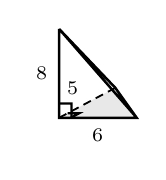
\begin{tikzpicture}[scale=0.68, every node/.style={font=\scriptsize, text=black}]
        \coordinate (O) at (-0.90,-0.68);
        \coordinate (A) at (0.55,-0.68);
        \coordinate (B) at (0.15,-0.12);
        \coordinate (V) at (-0.90,0.98);
        \fill[gray!18] (O) -- (A) -- (B) -- cycle;
        \draw[black, line width=0.9pt] (V) -- (O) -- (A) -- (B) (V) -- (A) (V) -- (B);
        \draw[black, line width=0.65pt, densely dashed] (O) -- (B);
        \rightbox[0.16]{V}{O}{A}
        \rightbox[0.15]{A}{O}{B}
        \node[left=0.5pt] at (-0.90,0.15) {$8$};
        \node[below=0.5pt] at (-0.18,-0.68) {$6$};
        \node[above left=-1pt] at (-0.40,-0.38) {$5$};
      \end{tikzpicture}
    \end{minipage}
  \end{tcolorbox}
\end{minipage}%
\hfill
\begin{minipage}[t]{9.4cm}\vspace{0pt}
  \begin{tcolorbox}[
    enhanced, sharp corners, colback=white, colframe=black, equal height group=rowEx12,
    boxrule=0.8pt, boxsep=3.5pt, top=9pt, bottom=9pt, left=5pt, right=5pt
  ]
    \textbf{គំរូទី \en{2} (ទំ.២២៤)៖ ពីរ៉ាមីតបាតចតុ.កែង ($7\times 5$; កម្ពស់ $h=6$)}\\[6pt]
    \begin{minipage}[c]{5.5cm}\raggedright
      $1.$ ផ្ទៃក្រឡាបាតចតុកោណកែង៖\\[5pt]
      \hspace*{0.15cm}$B = 7 \times 5 = \blank{1.2cm}$\\[7pt]
      $2.$ មាឌពីរ៉ាមីត ($h = 6$)៖\\[5pt]
      \hspace*{0.15cm}$V = \dfrac{1}{3} B \cdot h = \dfrac{1}{3}\times \blank{1.0cm}\times 6$\\[5pt]
      \hspace*{0.45cm}$= \blank{1.4cm}$ ឯកតាមាឌ ។
    \end{minipage}%
    \hfill
    \begin{minipage}[c]{2.8cm}
      \centering
      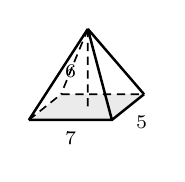
\begin{tikzpicture}[scale=0.68, every node/.style={font=\scriptsize, text=black}]
        \coordinate (V) at (0,1.02);
        \coordinate (A) at (-1.10,-0.68);
        \coordinate (B) at (0.45,-0.68);
        \coordinate (C) at (1.05,-0.20);
        \coordinate (D) at (-0.50,-0.20);
        \coordinate (O) at (0,-0.44);
        \fill[gray!16] (A) -- (B) -- (C) -- (D) -- cycle;
        \draw[black, line width=0.9pt] (A) -- (B) -- (C) (V) -- (A) (V) -- (B) (V) -- (C);
        \draw[black, line width=0.6pt, densely dashed] (A) -- (D) -- (C) (V) -- (D) (V) -- (O);
        \node[below=0.5pt] at (-0.32,-0.68) {$7$};
        \node[below right=-1pt] at (0.78,-0.46) {$5$};
        \node[left=0.5pt] at (0,0.22) {$6$};
      \end{tikzpicture}
    \end{minipage}
  \end{tcolorbox}
\end{minipage}

\vspace{21pt}
% --- E3 Explain: Formula Summary & Misconception Guard (h vs d) ---
\secbar{ផ្នែកទី២ ៖ សង្ខេបរូបមន្តមាឌពីរ៉ាមីត និងការបែងចែកកម្ពស់កែង $h$ ពីអាប៉ូតែម $d$ \enbf{(E3 - Explain)}}{សង្ខេបរួមគ្នា \en{6 min}}

\begin{tcolorbox}[
  enhanced, sharp corners, colback=white, colframe=black,
  boxrule=0.9pt, boxsep=5pt, top=11pt, bottom=11pt, left=6pt, right=6pt
]
  {\renewcommand{\arraystretch}{2.18}\footnotesize
  \begin{tabular}{|L{4.80cm}|L{5.60cm}|L{6.70cm}|}
    \hline
    \cellcolor{headgray}\textbf{រង្វាស់នៃពីរ៉ាមីត} & \cellcolor{headgray}\textbf{រូបមន្តគណនា} & \cellcolor{headgray}\textbf{ធាតុកម្ពស់ដែលត្រូវប្រើ (កុំច្រឡំ!)} \\
    \hline
    $1.$ មាឌនៃពីរ៉ាមីតទូទៅ ($V$) & $V = \dfrac{1}{\blank{0.7cm}} \times \blank{0.9cm} \times \blank{0.9cm}$ & ត្រូវប្រើ \textbf{កម្ពស់កែង $h$} (ទម្លាក់កែងពីកំពូលមកប្លង់បាត) \\
    \hline
    $2.$ ផ្ទៃក្រឡាខាងពីរ៉ាមីតនិយ័ត ($S_l$) & $S_l = \dfrac{1}{2} P \cdot d$ & ប្រើ \textbf{អាប៉ូតែមមុខខាង $d$} (កម្ពស់លើមុខត្រីកោណខាង) \\
    \hline
    $3.$ ស្ពានពីតាករ (បាតការេជ្រុង $a$) & $h = \sqrt{d^2 - \left(\dfrac{a}{2}\right)^2}$ & បើប្រាប់អាប៉ូតែម $d$ ត្រូវគណនារក $h$ សិន មុនគណនា $V$! \\
    \hline
  \end{tabular}}\\[10pt]
  $\bullet$ \textbf{ធនាគារហេតុផល៖}
  \cnum{1} $B =$ ផ្ទៃក្រឡាបាតពហុកោណ \;\textbar\;
  \cnum{2} $h = \sqrt{d^2-(a/2)^2}$ ជាកម្ពស់កែង \;\textbar\;
  \cnum{3} $V = \dfrac{1}{3}B\cdot h$ \;\textbar\;
  \cnum{4} សូលីតផ្សំ៖ $V = V_{\text{ព្រីស}} + V_{\text{ពីរ៉ាមីត}}$
\end{tcolorbox}

\newpage

% ============================================================================
% ទំព័រទី ២៖ E4 (ប្រតិបត្តិ ក និង ខ ទំ.២២៥) + E5 (បកស្រាយប៉មទី១៧ & Exit Check) + កិច្ចការផ្ទះ
% ============================================================================

\secbar{ផ្នែកទី៣ ៖ អនុវត្តលំហាត់ប្រតិបត្តិ ក និង ខ ទំព័រ ២២៥ \enbf{(E4 - Elaborate)}}{អនុវត្ត \en{10 min}}

\noindent
\begin{minipage}[t]{9.4cm}\vspace{0pt}
  \begin{tcolorbox}[
    enhanced, sharp corners, colback=white, colframe=black, equal height group=rowE4,
    boxrule=0.85pt, boxsep=3.5pt, top=7pt, bottom=7pt, left=5.5pt, right=5.5pt
  ]\raggedright
    \textbf{៣.ក ប្រតិបត្តិ ក (ទំ.២២៥ — លំហាត់គំរូបន្ថយជំហាន)៖}\\
    គណនាមាឌពីរ៉ាមីតបាតការេជ្រុង $a=14$ និងអាប៉ូតែម $d=25$៖
    \begin{center}
      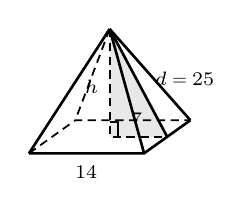
\begin{tikzpicture}[scale=0.84, every node/.style={font=\scriptsize, text=black}]
        \coordinate (V) at (0,1.18);
        \coordinate (A) at (-1.22,-0.70);
        \coordinate (B) at (0.52,-0.70);
        \coordinate (C) at (1.22,-0.20);
        \coordinate (D) at (-0.52,-0.20);
        \coordinate (O) at (0,-0.45);
        \coordinate (M) at (0.87,-0.45);
        \fill[gray!18] (V) -- (O) -- (M) -- cycle;
        \draw[black, line width=0.95pt] (A) -- (B) -- (C) (V) -- (A) (V) -- (B) (V) -- (C);
        \draw[black, line width=0.65pt, densely dashed] (A) -- (D) -- (C) (V) -- (D);
        \draw[black, line width=0.85pt, densely dashed] (V) -- (O) -- (M);
        \draw[black, line width=0.95pt] (V) -- (M);
        \rightbox[0.14]{V}{O}{M}
        \node[below=1pt] at (-0.35,-0.70) {$14$};
        \node[above=0.5pt] at (0.42,-0.45) {$7$};
        \node[left=0.5pt] at (0,0.30) {$h$};
        \node[right=1pt] at (0.50,0.42) {$d=25$};
      \end{tikzpicture}
    \end{center}
    $1.$ កន្លះជ្រុងបាត៖ $\dfrac{a}{2} = \dfrac{14}{2} = 7$ \;\textbar\; កម្ពស់កែងតាមពីតាករ \cnum{2}៖\\[3.5pt]
    \hspace*{0.15cm}$h = \sqrt{25^2 - 7^2} = \sqrt{625 - \blank{0.9cm}} = \sqrt{\blank{1.1cm}} = \blank{1.0cm}$\\[5pt]
    $2.$ ផ្ទៃក្រឡាបាតការេ \cnum{1}៖ $B = 14^2 = \blank{1.4cm}$\\[5pt]
    $3.$ មាឌពីរ៉ាមីត \cnum{3}៖ $V = \dfrac{1}{3}\times \blank{1.1cm}\times \blank{1.0cm} = \blank{1.5cm}$
  \end{tcolorbox}
\end{minipage}%
\hfill
\begin{minipage}[t]{9.4cm}\vspace{0pt}
  \begin{tcolorbox}[
    enhanced, sharp corners, colback=white, colframe=black, equal height group=rowE4,
    boxrule=0.85pt, boxsep=3.5pt, top=7pt, bottom=7pt, left=5.5pt, right=5.5pt
  ]\raggedright
    \textbf{៣.ខ ប្រតិបត្តិ ខ (ទំ.២២៥ — ធ្វើដោយខ្លួនឯង)៖}\\
    គណនាមាឌពីរ៉ាមីតបាតការេជ្រុង $a=10$ និងអាប៉ូតែម $d=13$៖
    \begin{center}
      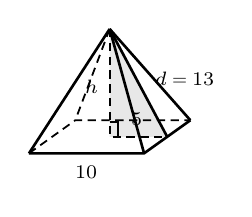
\begin{tikzpicture}[scale=0.84, every node/.style={font=\scriptsize, text=black}]
        \coordinate (V) at (0,1.18);
        \coordinate (A) at (-1.22,-0.70);
        \coordinate (B) at (0.52,-0.70);
        \coordinate (C) at (1.22,-0.20);
        \coordinate (D) at (-0.52,-0.20);
        \coordinate (O) at (0,-0.45);
        \coordinate (M) at (0.87,-0.45);
        \fill[gray!18] (V) -- (O) -- (M) -- cycle;
        \draw[black, line width=0.95pt] (A) -- (B) -- (C) (V) -- (A) (V) -- (B) (V) -- (C);
        \draw[black, line width=0.65pt, densely dashed] (A) -- (D) -- (C) (V) -- (D);
        \draw[black, line width=0.85pt, densely dashed] (V) -- (O) -- (M);
        \draw[black, line width=0.95pt] (V) -- (M);
        \rightbox[0.14]{V}{O}{M}
        \node[below=1pt] at (-0.35,-0.70) {$10$};
        \node[above=0.5pt] at (0.42,-0.45) {$5$};
        \node[left=0.5pt] at (0,0.30) {$h$};
        \node[right=1pt] at (0.50,0.42) {$d=13$};
      \end{tikzpicture}
    \end{center}
    $1.$ កន្លះជ្រុងបាត៖ $\dfrac{a}{2} = \blank{0.8cm}$ \;\textbar\; កម្ពស់កែងតាមពីតាករ \cnum{2}៖\\[3.5pt]
    \hspace*{0.15cm}$h = \sqrt{13^2 - (\blank{0.7cm})^2} = \sqrt{\blank{1.1cm} - \blank{0.9cm}} = \blank{1.0cm}$\\[5pt]
    $2.$ ផ្ទៃក្រឡាបាតការេ \cnum{1}៖ $B = 10^2 = \blank{1.4cm}$\\[5pt]
    $3.$ មាឌពីរ៉ាមីត \cnum{3}៖ $V = \dfrac{1}{3}\times \blank{1.1cm}\times \blank{1.0cm} = \blank{1.5cm}$
  \end{tcolorbox}
\end{minipage}

\vspace{14pt}
% --- E5 Evaluate: Resolve E1 Architectural Tower (Ex #17 p. 229) + Exit Check ---
\secbar{ផ្នែកទី៤ ៖ វាយតម្លៃ \enbf{---} បកស្រាយបេសកកម្ម \enbf{E1 (}លំហាត់ទី១៧ ទំ\enbf{.}២២៩\enbf{)} និង \enbf{Exit Check (E5)}}{ធ្វើដោយឯករាជ្យ \en{10 min}}

\noindent
\begin{minipage}[t]{10.1cm}\vspace{0pt}
  \begin{tcolorbox}[
    enhanced, sharp corners, colback=white, colframe=black, equal height group=rowE5,
    boxrule=0.85pt, boxsep=3.5pt, top=7.5pt, bottom=7.5pt, left=5.5pt, right=5.5pt
  ]\raggedright
    \textbf{៤.ក បកស្រាយបេសកកម្មទី១ — មាឌប៉មលំហាត់ទី១៧ (ទំ.២២៩)៖}\\[5.5pt]
    $1.$ ផ្ទៃបាតការេ៖ $B = 5\times 5 = \blank{1.1cm}\unit{m}^2$\\[5pt]
    $2.$ មាឌតួប៉មរាងប្រអប់កែង ($h_1 = 20\unit{m}$)៖\\[3.5pt]
    \hspace*{0.15cm}$V_1 = B \cdot h_1 = \blank{1.0cm} \times 20 = \blank{1.4cm}\unit{m}^3$\\[5pt]
    $3.$ មាឌដំបូលរាងពីរ៉ាមីត ($h_2 = 24 - 20 = \blank{0.8cm}\unit{m}$)៖\\[3.5pt]
    \hspace*{0.15cm}$V_2 = \dfrac{1}{3} B \cdot h_2 = \dfrac{1}{3}\times \blank{1.0cm}\times \blank{0.8cm} = \blank{1.6cm}\unit{m}^3$\\[5pt]
    $4.$ មាឌសរុបនៃប៉ម \cnum{4}៖ $V = V_1 + V_2 = \blank{2.2cm}\unit{m}^3$
  \end{tcolorbox}
\end{minipage}%
\hfill
\begin{minipage}[t]{8.7cm}\vspace{0pt}
  \begin{tcolorbox}[
    enhanced, sharp corners, colback=white, colframe=black, equal height group=rowE5,
    boxrule=0.85pt, boxsep=3.5pt, top=7.5pt, bottom=7.5pt, left=5.5pt, right=5.5pt
  ]\raggedright
    \textbf{៤.ខ សំណួរត្រួតពិនិត្យរហ័ស (\en{Exit Check})៖}\\
    គូសវង់ជុំវិញអក្សរនៃចម្លើយត្រឹមត្រូវតែមួយគត់៖\\[6pt]
    \textbf{សំណួរទី១៖} បើព្រីសនិងពីរ៉ាមីតមានបាត $B$ និងកម្ពស់ $h$ ស្មើគ្នា ហើយ $V_{\text{ព្រីស}} = 90\unit{cm}^3$ នោះ $V_{\text{ពីរ៉ាមីត}}$ ស្មើនឹង៖\\[2.5pt]
    \hspace*{0.15cm}\textbf{ក.} $45\unit{cm}^3$ \hspace{0.55cm} \textbf{ខ.} $30\unit{cm}^3$ \hspace{0.55cm} \textbf{គ.} $270\unit{cm}^3$\\[6.5pt]
    \textbf{សំណួរទី២ (ទី១០ក ទំ.២២៨)៖} ពីរ៉ាមីតមានផ្ទៃបាត $B = 100\unit{cm}^2$ និងកម្ពស់ $VO = 12\unit{cm}$ មានមាឌស្មើនឹង៖\\[2.5pt]
    \hspace*{0.15cm}\textbf{ក.} $400\unit{cm}^3$ \hspace{0.45cm} \textbf{ខ.} $1200\unit{cm}^3$ \hspace{0.45cm} \textbf{គ.} $600\unit{cm}^3$\\[6.5pt]
    \textbf{សំណួរទី៣៖} ពីរ៉ាមីតបាតការេជ្រុង $6\unit{cm}$ ($B=36\unit{cm}^2$) អាប៉ូតែម $d=5\unit{cm}$ និងកម្ពស់កែង $h=4\unit{cm}$ មានមាឌ៖\\[2.5pt]
    \hspace*{0.15cm}\textbf{ក.} $\frac{1}{3}(36)(5)$ \hspace{0.35cm} \textbf{ខ.} $36\times 4$ \hspace{0.35cm} \textbf{គ.} $\frac{1}{3}(36)(4)=48\unit{cm}^3$
  \end{tcolorbox}
\end{minipage}

\vspace{14pt}
% --- Step 5 Homework Box ---
\secbar{ផ្នែកទី៥ ៖ កិច្ចការផ្ទះ និងបណ្ដាំផ្ញើ \enbf{(}ទំព័រ ២២៨ លំហាត់ទី៨ង និងទំព័រ ២៣០ លំហាត់ទី២១\enbf{)}}{ធ្វើនៅផ្ទះក្នុងសៀវភៅសរសេរ}

\begin{tcolorbox}[
  enhanced, sharp corners, colback=panelgray, colframe=black,
  boxrule=0.85pt, boxsep=3.5pt, top=7.5pt, bottom=7.5pt, left=6pt, right=6pt
]
  \begin{minipage}[c]{14.0cm}\raggedright
    $1.$ \textbf{លំហាត់ទី៨ ង (ទំ.២២៨ — រូបខាងស្ដាំ)៖} គណនាមាឌនៃសូលីតផ្សំពីគូបទ្រនុង $20\unit{ft}$ និងពីរ៉ាមីតកំពូលដែលមានកម្ពស់កែង $15\unit{ft}$ ។\\[4.5pt]
    $2.$ \textbf{លំហាត់ទី២១ (ទំ.២៣០)៖} គណនាមាឌពីរ៉ាមីតចតុមុខនិយ័តដែលមានអង្កត់ទ្រូងបាតការេស្មើ $10\unit{dm}$ និងទ្រនុងខាងស្មើ $13\unit{dm}$ (ណែនាំ៖ ផ្ទៃការេ $B = \frac{10^2}{2} = 50\unit{dm}^2$, កន្លះអង្កត់ទ្រូងបាត $= 5\unit{dm}$ និង $h = \sqrt{13^2-5^2}$) ។\\[4.5pt]
    $3.$ \textbf{អានមេរៀនបន្ទាប់៖} ១៧.៤ ការគណនាមាឌនៃកោន (ទំ.២២៥\,\en{--}\,២២៦) ។
  \end{minipage}%
  \hfill
  \begin{minipage}[c]{3.9cm}
    \centering
    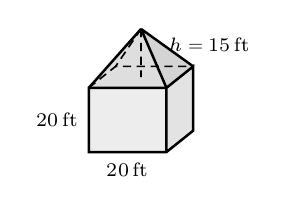
\begin{tikzpicture}[scale=0.68, every node/.style={font=\scriptsize, text=black}]
      % លំហាត់ទី៨ង៖ គូប 20ft + ពីរ៉ាមីត h=15ft
      \coordinate (A) at (-1.00,-0.85);
      \coordinate (B) at (0.45,-0.85);
      \coordinate (C) at (0.95,-0.45);
      \coordinate (A1) at (-1.00,0.35);
      \coordinate (B1) at (0.45,0.35);
      \coordinate (C1) at (0.95,0.75);
      \coordinate (D1) at (-0.50,0.75);
      \coordinate (V) at (-0.025,1.45);
      \coordinate (O1) at (-0.025,0.55);
      \fill[gray!14] (A) -- (B) -- (B1) -- (A1) -- cycle;
      \fill[gray!22] (B) -- (C) -- (C1) -- (B1) -- cycle;
      \fill[gray!26] (A1) -- (B1) -- (V) -- cycle;
      \fill[gray!34] (B1) -- (C1) -- (V) -- cycle;
      \draw[black, line width=0.9pt] (A) -- (B) -- (C) -- (C1) -- (B1) -- (A1) -- cycle (B) -- (B1);
      \draw[black, line width=0.9pt] (V) -- (A1) (V) -- (B1) (V) -- (C1);
      \draw[black, line width=0.6pt, densely dashed] (A1) -- (D1) -- (C1) (V) -- (D1) (V) -- (O1);
      \node[below=0.5pt] at (-0.28,-0.85) {$20\unit{ft}$};
      \node[left=0.5pt] at (-1.00,-0.25) {$20\unit{ft}$};
      \node[right=1pt] at (0.28,1.15) {$h=15\unit{ft}$};
    \end{tikzpicture}
  \end{minipage}
\end{tcolorbox}

\end{document}
